% HMC Math dept HW template example
% v0.04 by Eric J. Malm, 10 Mar 2005
\documentclass[12pt,letterpaper,boxed,cm]{hmcpset}

% set 1-inch margins in the document
\usepackage[margin=1in]{geometry}
\usepackage{mathtools}
\usepackage{mathrsfs}
% include this if you want to import graphics files with /includegraphics
\usepackage{graphicx}
\usepackage{cases}
\usepackage{hyperref}
\usepackage{siunitx}
\usepackage{tikz}
\usepackage{cases}
\usepackage{mathalfa}
\usetikzlibrary{arrows}

% info for header block in upper right hand corner
\name{Name: ~~~~~~~~~~~~~~~~~~~~~~~~~~~~~~~}
\class{Physics 51}
\assignment{Homework \#22}
\duedate{December 1, 2016}

\newcommand{\ev}[2]{\Big|_{#1}^{#2}}
\newcommand{\evv}[2]{\Big|_{#1}^{#2}}
\newcommand{\set}[1]{\left\{#1\right\}}
\newcommand{\s}[1]{\sqrt{#1}}
\newcommand{\f}[2]{\frac{#1}{#2}}
\newcommand{\p}[2]{\frac{\partial #1}{\partial #2}}
\providecommand{\t}[1]{\text{#1}}
\providecommand{\span}[1]{\text{span}\left(#1\right)}
\providecommand{\set}[1]{\left\{#1\right\}}
\providecommand{\l}[0]{\left}
\providecommand{\r}[0]{\right}
\newcommand{\m}[1]{\begin{matrix}#1\end{matrix}}
\newcommand{\bm}[1]{\begin{bmatrix}#1\end{bmatrix}}
\renewcommand{\bf}[1]{\mathbf{#1}}
\newcommand{\pn}[1]{\left( #1 \right)}
\newcommand{\abs}[1]{\left| #1 \right|}
\newcommand{\bk}[1]{\left[ #1 \right]}
\newcommand{\cis}[1]{\pn{\cos\pn{#1} + i\sin\pn{#1}}}
\newcommand{\cisi}[1]{\pn{\cos\pn{#1} - i\sin\pn{#1}}}
\renewcommand{\Im}[1]{\text{Im}\pn{#1}}
\renewcommand{\Re}[1]{\text{Re}\pn{#1}}
\renewcommand{\k}[0]{\f{1}{4\pi\epsilon_0}}
\renewcommand{\part}[1]{\vspace{1em}\noindent(#1)}

\makeatletter
\renewcommand*\env@matrix[1][*\c@MaxMatrixCols c]{%
  \hskip -\arraycolsep
  \let\@ifnextchar\new@ifnextchar
  \array{#1}}
\makeatother
\begin{document}
\problemlist{Townsend 1.\{19,24,26\}}

\begin{problem}[Townsend 1.19]
	 Express the complex number $z_1 = (\s{3} + i)/ 2$ in the form $re^{i\phi}$. What about $z_2 = (1 + \s{3}i)/2$? If these complex numbers are the probability amplitudes for photons to be detected, what is the probability in each case?
\end{problem}
\begin{solution}
\end{solution}
\newpage

\begin{problem}[Townsend 1.24]
	\begin{enumerate}
		\item[(a)] Show that the probability of a photon of wavelength $\lambda$ being reflected from a thin layer of glass of thickness $d$ at normal incidence is given by
		\[
			P = 0.16\sin^2\pn{2\pi d/\lambda'}
		\]
		where $\lambda'$ is the wavelength of light in glass, i.e., $\lambda' = \lambda/n$, where $n$ is the index of refraction of glass. \textit{Note}: In this calculation assume that the magnitude of the amplitude for reflection from the top or the bottom surface of the glass is 0.2 and that there is an additional phase change of $\pi$ in the reflection from the top surface. Also assume that amplitudes that arise from multiple reflections between the top and bottom surfaces of the glass can be neglected in your calculation. Given the result of Problem 1.23, it is okay to approximate the magnitude of the amplitude for transmission as one. \textit{Hint}: What extra distance does light travel in being reflected from the bottom surface relative to the top surface? (Use $\lambda = \SI{706}{nm}$).
		\item[(b)] In \textit{QED: The Strange Theory of Light and Matter} Feynman states that as the thickness of a thin layer of glass increases from zero thickness, the probability of reflection first reaches a value of 0.16 when the thickness of the layer of glass is 5 millionths of an inch. What index of refraction is being assumed? Take the wavelength of the light in air to be the same as you determined in Problem 1.22. 
		\item[(c)] What is the minimum value of $d$ necessary to produce zero reflection?
	\end{enumerate}
	\textit{Note: For this problem, use} $\lambda = \SI{706}{nm}$.
\end{problem}
\begin{solution}
\end{solution}
\newpage

\begin{problem}[Townsend 1.26]
	 Assume that the first beam splitter at A in the Mach-Zehnder interferometer (Fig. 1.23) is a ``third-silvered mirror," that is, a mirror that reflects one-third the light and transmits two-thirds. The two mirrors at B and C reflect 100\% of the light. and the second beam splitter at D is a traditional half-silvered mirror that reflects one-half the light and transmits one-half. The probability of detecting a photon in either photomultiplier $\text{PM}_1$ or $\text{PM}_2$ varies with the position of the movable mirror, say mirror B. Determine the maximum probability and the minimum probability of obtaining a count in, say, $\text{PM}_1$. What is the visibility
	 \[
	 	V = \f{P_{\text{max}} - P_{\text{min}}}{P_{\text{max}} + P_{\text{min}}}.
	 \]
	of the interference fringes, where $P_{\text{max}}$ and $P_{\text{min}}$ are the maximum and minimum probabilities, respectively, that a photon is counted by the detector, as the position of the movable mirror varies? Note: In the experiment of Aspect et al. described in Section 1.5 the visibility of the fringes is $0.987 \pm 0.005$.
	 \begin{center}
	 	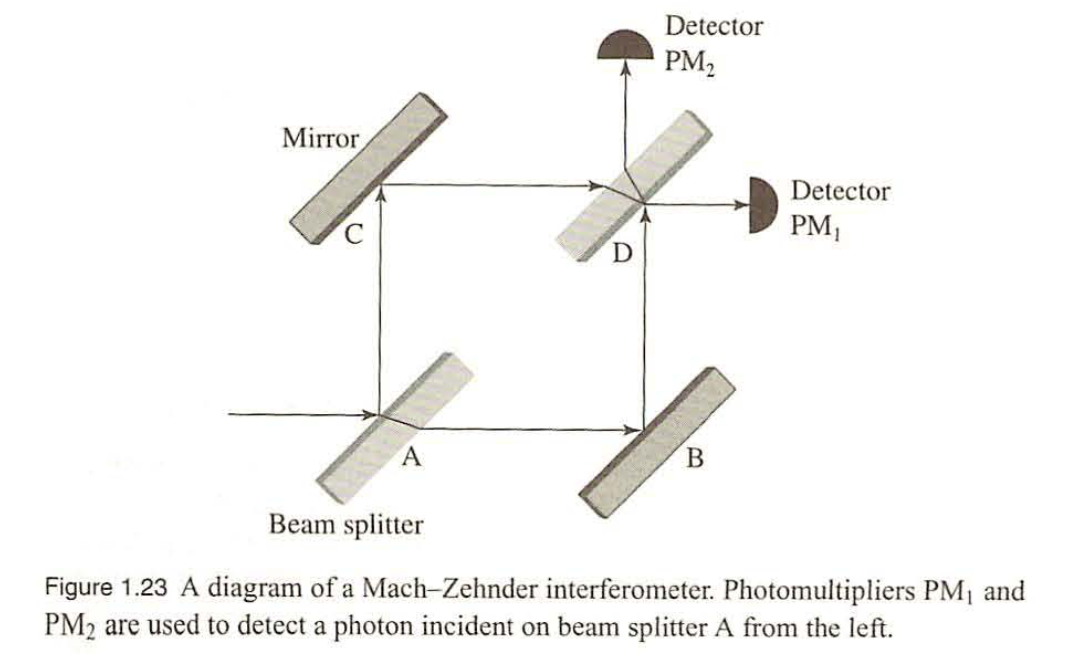
\includegraphics[scale=0.6]{pic01.png}	
	 \end{center}
\end{problem}
\begin{solution}
\end{solution}
\end{document}